\documentclass[12pt]{article}
\usepackage{amsfonts}
\usepackage{amsmath}
\usepackage{bm}
\usepackage{bbm}
\usepackage{graphicx}
\usepackage{geometry}[margin=1in]
\usepackage{subcaption}
\usepackage{algorithm}
\usepackage{algorithmic}


\title{Regionally Additive Models: Explainable-by-design models minimizing feature interactions}

\newcommand{\Rd}{\mathbb{R}^d}
\newcommand{\xb}{\mathbf{x}}
\newcommand{\xc}{\mathbf{x_c}}
\newcommand{\fxc}{f^{(\xc)}}
\newcommand{\fxs}{f^{(x_s)}}
\newcommand{\Xcal}{\mathcal{X}}
\newcommand{\Ycal}{\mathcal{Y}}
\newcommand{\when}[1]{\mathbbm{1}_{#1}}

\author{Vasilis Gkolemis}


\begin{document}
\maketitle

\begin{abstract}
Generalized Additive Models (GAMs) are a popular class of explainable-by-design models that are widely used in practice.
GAMs are based on the assumption that the effect of each feature on the target is independent of the values of the
other features, however, in cases where this assumption is violated they may lead to poor performance.
To address this limitation we propose Regionally Additive Models (RAMs), a novel class of explainable-by-design models,
that fits multiple GAMs to subregions of the feature space where interactions are minimized.
Our approach consists of two steps: first, we fit a black-box model and we identify the subregions where the black-box model is nearly locally additive,
i.e., where the effect of each feature on the target is independent of the values of the other features.
Secondly, we train a GAM specifically for each identified subregion.

We show that RAMs are more expressive than GAMs while they are still interpretable.

\end{abstract}

\section{Introduction and Related Work}


% Paragraph for Motivating about Regionally Additive Models
Generalized Additive Models (GAMs) are a widely recognized class of explainable-by-design models.
Their popularity stems from their seamless interpretability; since they are a linear (additive) combination of univariate functions,
$f(\xb) = c + \sum_{s=1}^D f_s(x_s)$, each individual univariate function can be readily visualized and comprehended in isolation.
However, the expressiveness of GAMs is limited when it comes to learn interactions between features.
To overcome this limitation, a family of models extends GAMs enabling pairwise interactions,
i.e., $f(\xb) = c + \sum_{s=1}^D f_s(x_s) + \sum_{s=1}^D \sum_{c \neq s} f_{sc}(x_s, x_c)$.
Pairwise interactions can also be visualized and understood in isolation, so these models also maintain their explainable-by-design nature.
Unfortunately, this does not hold for any interaction that involves more than two features, thus, the expressiveness of GAMs is limited to capturing up to two-feature interactions.

% Paragraph for Motivating about Regionally Additive Models
To overcome this limitation, we propose Regionally Additive Models (RAMs), a novel class of explainable-by-design models,
that fits multiple GAMs to subregions of the feature space where interactions are minimized.
Our approach consists of a three-step pipeline.
First, we fit a black-box model to capture all high-order interactions.
Second, we identify the subregions where the black-box model is nearly locally additive.
Finally, we train a GAM specifically for each identified subregion.

\section{Motivation}

Consider the black-box function
\(f(\xb) = 8x_2\when{x_1 > 0}\when{x_3=0}\) with \(x_1, x_2 \sim \mathcal{U}(-1,1)\) and \(x_3 \sim Bernoulli(0,1)\).
The black-box function $f$ involves a three-term interaction term which cannot be captured by a GAM (Figure~\ref{subfig:global_gam}).
However, if splitting the input space in two subregions we observe that $f$ is locally additive
in each one, i.e.,
%
\begin{equation}
    f(\xb) = \begin{cases} 8x_2 & \text{if } x_1 > 0 \text{ and } x_3 = 0 \\ 0 & \text{otherwise} \end{cases}
\end{equation}
%
and a Regionally Additive Model (RAM)

\begin{equation}
f^{\mathtt{RAM}}(\xb) = c + \sum_{s=1}^D f^{\mathtt{RAM}}_s(x_s) = c + \sum_{s=1}^D \sum_k f_{sk}(x_s) \when{\xc \in \mathcal{R}_{sk}}
\end{equation}
%
can perfectly capture the black-box function.
In this case, $f^{\mathtt{RAM}}_1(x_1)$, $f^{\mathtt{RAM}}_3(x_3)$ are zero and $f^{\mathtt{RAM}}_2(x_2)$ has two cases;
$f_{21}(x_2) = 8x_2$ for $\mathcal{R}_{21} = \{x_1 > 0 \text{ and } x_3 = 0\}$ and $f_{22}(x_2) = 0$ for $\mathcal{R}_{22} = \{x_1 \leq 0 \text{ or } x_3 = 1\}$.
Importantly, RAM's expressiveness does not come at the expense of interpretability.
We can still visualize and comprehend each univariate function in isolation, exactly as we would do with a GAM,
with the only difference being that we have to consider the subregions where each univariate function is active, as we observe in
Figures~\ref{subfig:regional_gam_1} and~\ref{subfig:regional_gam_2}.

The key idea and the main challenge of RAMs is to identify the subregions where the black-box function is locally
closer to additive.
Each split adds a new univariate function to the final model and enforces the user to interpret more univariate functions to understand the model behavior.
Thus, the number of splits should be kept as small as possible.


\begin{figure}[htbp]
    \centering
    \begin{subfigure}{0.32\textwidth}
        \centering
        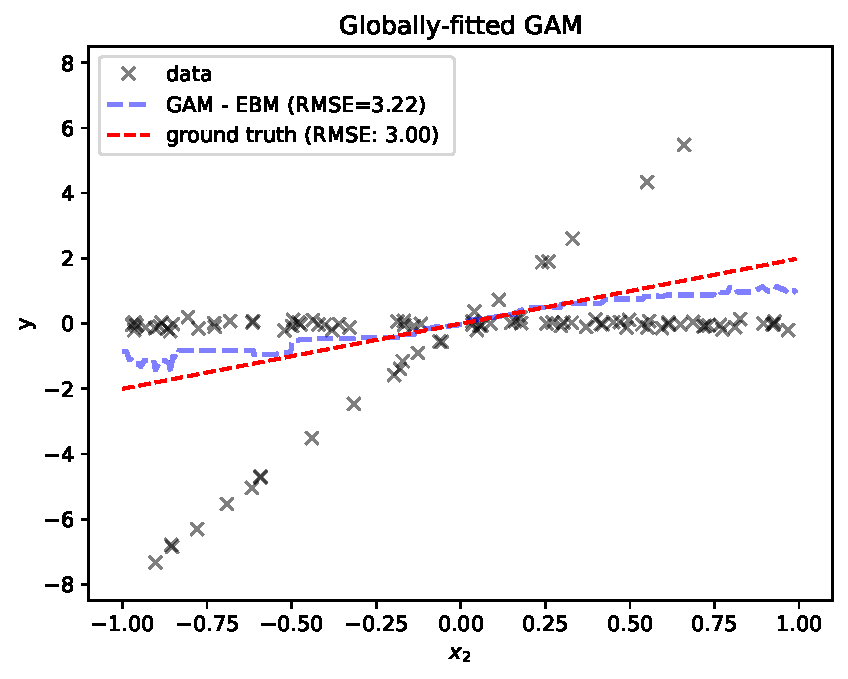
\includegraphics[width=\textwidth]{figures/global_GAM.pdf}
        \caption{$f_2(x_2)$}
        \label{subfig:global_gam}
    \end{subfigure}
    \begin{subfigure}{0.32\textwidth}
        \centering
        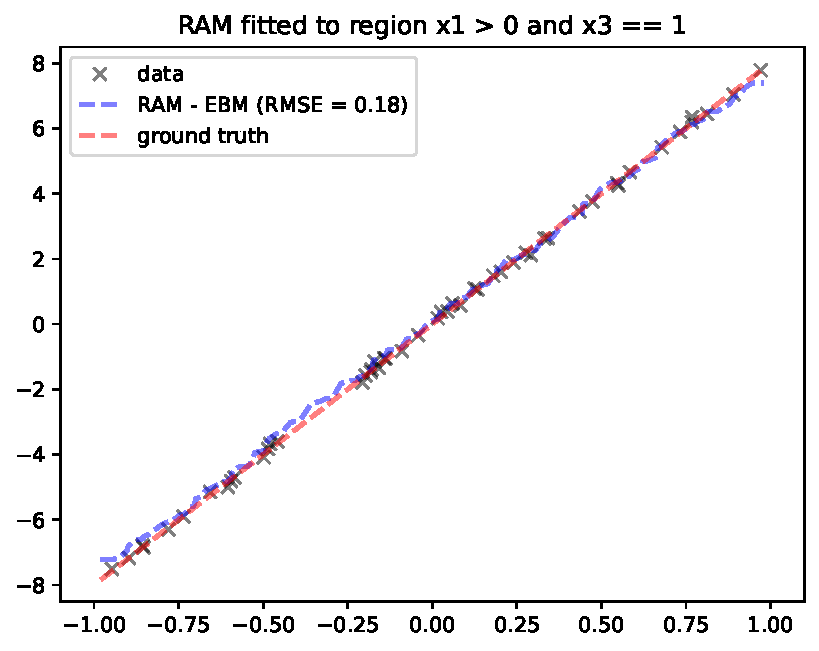
\includegraphics[width=\textwidth]{figures/regional_gam_subreg_1.pdf}
        \caption{$f_2(x_2) \when{x_1 > 0} \when{x_3=0}$}
        \label{subfig:regional_gam_1}
    \end{subfigure}
    \begin{subfigure}{0.32\textwidth}
        \centering
        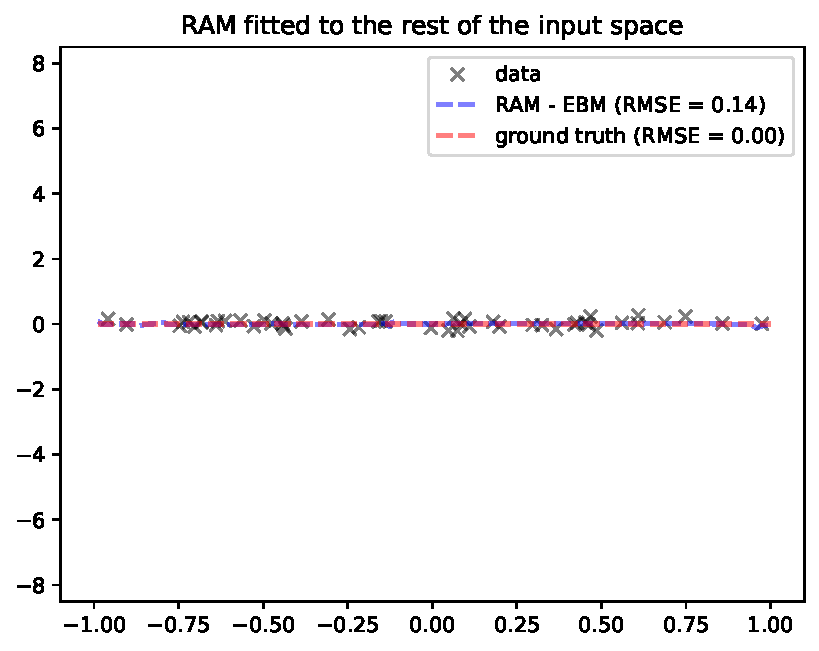
\includegraphics[width=\textwidth]{figures/regional_gam_subreg_2.pdf}
        \caption{$f_2(x_2) \when{x_1 \leq 0 \text{ or } x_3 = 1}$}
        \label{subfig:regional_gam_2}
    \end{subfigure}
    \caption{Caption for the entire figure}
    \label{fig:ram_example}
\end{figure}


\section{The Regionally Additive Models (RAMs) Framework}


\begin{algorithm}
\caption{Regionally Additive Models (RAMs)}
\label{alg:ram}
\begin{algorithmic}[1]
\REQUIRE Dataset $\mathcal{D} = \{(\mathbf{x}_i, y_i)\}_{i=1}^n$, black-box model $f(\mathbf{x})$, regional effect method $\mathcal{R}$, RAM $f^{\mathtt{RAM}}(\mathbf{x})$
\STATE Fit a black-box model $f(\mathbf{x})$ to $\mathcal{D} = \{(\mathbf{x}_i, y_i)\}_{i=1}^n$
\STATE Identify the subregions $\mathcal{R}_{sk}$ using a regional effect method
\STATE Define the RAM $f^{\mathtt{RAM}}(\mathbf{x}) = c + \sum_{s=1}^D f^{\mathtt{RAM}}_s(x_s) = c + \sum_{s=1}^D \sum_k f_{sk}(x_s) \when{\xc \in \mathcal{R}_{sk}}$
\STATE Fit the univariate functions $f_{sk}(x_s)$ for each $s$ and $k$.
\end{algorithmic}
\end{algorithm}

RAM is a framework for fitting explainable-by-design models that are expressive enough to capture any interaction.
This is achieved using a pipeline that consists of a sequence of steps (Algorithm~\ref{alg:ram}).
In the first step, we fit a black-box model $f$ to the data.
The black-box model can be any model that is expressive enough to accurately fit the data.
For example, we can use a random forest or a neural network.
In the second step, we identify the subregions where the black-box model is nearly locally additive.
This is achieved using a regional effect method $\mathcal{R}$.
For example, we can use REPID (add citation) or any method presented by \citet{ribeiro2016should}.
At section \ref{sec:regional_effect_methods} we present a regional effect method based on the ALE plot.
This step defines the form of the final model as defined in equation \ref{eq:ram}.
Finally, we fit a GAM to the identified subregions, using any GAM model.

\subsection{Background}

Let \(\Xcal \in \Rd\) be the \(d\)-dimensional feature space, \(\Ycal\) the target space and \(f(\cdot) : \Xcal \rightarrow \Ycal\) the black-box function.  We use index \(s \in \{1, \ldots, d\}\) for the feature of interest and \(c = \{1, \ldots, d\} - s\) for the rest.
For convenience, we use \((x_s, \xc)\) to refer to \((x_1, \cdots , x_s, \cdots, x_D)\) and, equivalently, \((X_s, X_c)\) instead of \((X_1, \cdots , X_s, \cdots, X_D)\) when we refer to random variables.
The training set \(\mathcal{D} = \{(\xb^i, y^i)\}_{i=1}^N\) is sampled
i.i.d.\ from the distribution \(\mathbb{P}_{X,Y}\).  Finally,
\(f^{\mathtt{<method>}}(x_s)\) denotes how \(\mathtt{<method>}\)
defines the feature effect and \(\hat{f}^{\mathtt{<method>}}(x_s)\)
how it estimates it from the training set.


\subsection{Identifying the Regions of Locally Additivity}

\subsection{Fitting the GAMs}

\section{Experiments}

\subsection{Synthetic Examples}

\subsection{Real-World Datasets}


\end{document}
